
% Include LaTeX packages
\documentclass[conference]{styles/acmsiggraph}
\usepackage{fullpage}
\usepackage{enumitem}
\usepackage{amsmath,amsthm,amssymb}
\usepackage{listings}
\usepackage{graphicx}
\usepackage{etoolbox}
\usepackage{verbatim}
\usepackage[dvipsnames]{xcolor}
\usepackage{fancyvrb}
\usepackage{hyperref}
\usepackage{menukeys}
\usepackage{booktabs}
\usepackage{mathtools} % mathtools builds on and extends amsmath package
% \setlength{\parskip}{0.4em}
% \pagestyle{myheadings}
% \pagenumbering{arabic}

\title{Assignment 1: Solutions \\ {IS711: Learning and Planning in Intelligent Systems}}
\author{SHI Jieke \\ jkshi.2022@phdcs.smu.edu.sg}
\pdfauthor{SHI Jieke}

\begin{document}
\maketitle
\vspace{-0.15cm}
\section{Question \#1}

\subsection{Answer to Question \#1.1}

We can formulate the problem with the following definitions:
The state space is the set of all possible configurations.
\begin{itemize}[itemsep=0.1em, leftmargin=*]
	\setlength{\itemsep}{0pt}
	\setlength{\parsep}{0pt}
	\setlength{\parskip}{0pt}
	\item \textbf{State representation}: A state can be represented by one or several piles. Each pile is represented by a stack of blocks denoted as color+label. For example, the Configuration 1 of this question is in the state of \{[\textit{Green A, Grey B, Orange A}], [\textit{Yellow B, Green C}]\}. There are five blocks available. The first block of each pile is the top and the last block is on the table.
	\item \textbf{State space}: The state space is the set of all possible configurations of piles.
	\item \textbf{Initial state}: \{[\textit{Green A, Grey B, Orange A}], [\textit{Yellow B, Green C}]\}.
	\item \textbf{Goal state}: \{[\textit{Green C, Grey B, Yellow B, Orange A, Green A}]\}.
	\item \textbf{Possible Operators}: denoting $x$ and $y$ as two blocks at the top of two piles, the possible operators are:
	\begin{itemize}
		\item \textit{Move(x, y)}: move the block $x$ to atop $y$.
		\item \textit{MoveToTable(x)}: move the block $x$ to the table.
	\end{itemize}
	\item \textbf{Path cost}: The cost of each call to operator \textit{Move(x, y)} is 1. The cost of each call to operator \textit{MoveToTable(x)} is determined by color, namely, Orange block costs 2, Gray block costs 3, Yellow block costs 1, Green block costs 4. The path cost is the sum of the costs of all calls to operators.
\end{itemize}

\subsection{Answer to Question \#1.2}

The heuristic function is $h(s) = \#blocks\_not\_in\_goal\_place (s)$, i.e., the number of blocks that do not arrive goal place in the state $s$. The heuristic function is admissible. When a block is not at the goal place, it costs at least 1 to call the operator \textit{Move} or more to call the \textit{MoveToTable}. Thus, for each state, $h(s)$ is always less than or equal to the actual cost to reach the goal state. 

The first four nodes of the search tree are shown as Figure



\section{Question \#2}

The trip with the least possible cost would need 6 large buses and 5 small buses.
The calculation using linear programming is as follows:
\begin{itemize}[leftmargin=*]
	\setlength{\itemsep}{0pt}
	\setlength{\parsep}{0pt}
	\setlength{\parskip}{0pt}
	\item \textbf{Variables}: $x_1$: the number of large buses; $x_2$: the number of small buses.
	\item \textbf{Objective}: Minimize rental costs, i.e.,
	\begin{equation}
		\min 800x_1 + 600 x_2
	\end{equation}
	\item \textbf{Constraints}: Subject to the following constraints:
	\begin{equation}
		\begin{aligned}
			& 50x_1 + 40x_2 \geq 500 \\
			& x_1 + x_2 \leq 11 \\
			& 0 \leq x_1 \leq 10 \\
			& 0 \leq x_2 \leq 8 \\
		\end{aligned}
	\end{equation}
	\item \textbf{Solution}: As shown in Figure~\ref{fig:2}, the optimal solution is $x_1 = 6$ and $x_2 = 5$. The minimum cost is $800 \times 6 + 600 \times 5 = 7800$.
	\begin{figure}[!h]
		\centering
		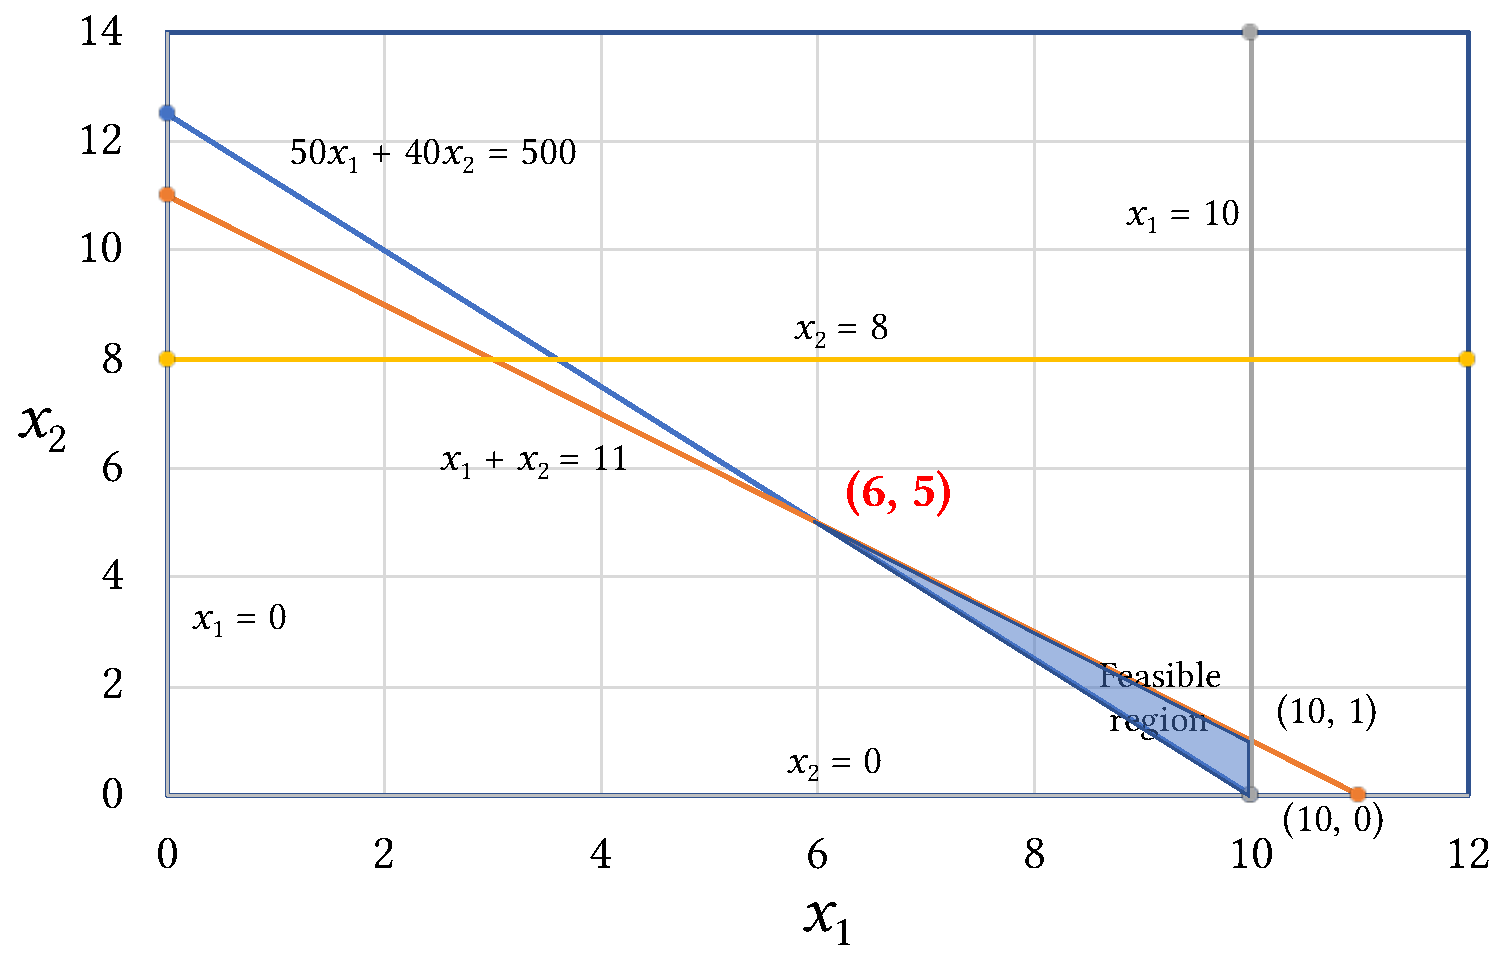
\includegraphics[width=0.7\textwidth]{figures/q2.pdf}
		\caption{Solution to Question \#2}
		\label{fig:2}
	\end{figure}
\end{itemize}

The drawbacks of linear programming are:
\begin{itemize}[leftmargin=*]
	\setlength{\itemsep}{0pt}
	\setlength{\parsep}{0pt}
	\setlength{\parskip}{0pt}
    \item To the above question, we can observe redundant computation in linear programming, i.e., if we remove the constraint $x_2\leq 8$, the answer will be unchanged. The other constraints are already sufficient conditions for the answer, but linear programming still needs to compute the redundant constraint $x_2\leq 8$.
    \item In the general cases of using linear programming, 
    \begin{itemize}[leftmargin=*]
        \item  When facing real-life problems, it is possible that the constraints may not be directly expressible as linear inequalities. Non-linear relations may be involved, e.g., $x_1^2 + x_2^2 \leq 100$;
        \item When solving linear programming, there is no guarantee of getting integer values. A non-integer valued solution will be meaningless to lots of problems.
        \item Linear programming can only handle single-objective problems, while real-life decision-making problems often have multiple objectives.
        \item The solution of linear programming can involve massive mathematical calculations. In some cases, the solution may not be available due to the complexity of the problem.
	\end{itemize}
\end{itemize}

\section{Question \#3}

I will play the game as the winning probability is $0.517 > 0.5$, and the expected value is $0.279 > 0$. The calculation is as follows:

For each round of rolling the dice, there exist $6^3$ possible outcomes. Among them, 
\begin{itemize}[leftmargin=*]
	\setlength{\itemsep}{0pt}
	\setlength{\parsep}{0pt}
	\setlength{\parskip}{0pt}
	\item There is 1 outcome whose total is 3. 
	\item There are 10 outcomes whose total is 6.
	\item There are 21 outcomes whose total is 8.
	\item There are 25 outcomes whose total is 9.
	\item There are 27 outcomes whose total is 11.
	\item There are 25 outcomes whose total is 12.
	\item There are 10 outcomes whose total is 15.
	\item There are 1 outcomes whose total is 18.
\end{itemize}

Therefore, the probability of winning \$1 in the first round is
\begin{equation}
	P(\text{winning \$1 in first round}) = \frac{1+21+27+10}{6^3} = \frac{59}{216} \approx 0.273
\end{equation}

The probability of losing \$1 in the first round is
\begin{equation}
	P(\text{losing \$1 in first round}) = \frac{25+1}{6^3} = \frac{26}{216} \approx 0.120
\end{equation}

% The probability of playing one more time is
% \begin{equation} 
% 	P(\text{playing one more time}) = 1- \frac{59}{216} - \frac{26}{216}  = \frac{131}{216} \approx 0.606
% \end{equation}

The probability of winning \$2 in the second round is
\begin{equation} 
	P(\text{winning \$2 in second round}) = (1- \frac{59}{216} - \frac{26}{216}) \times \frac{10+25+27+25}{6^3} = \frac{11397}{46656} \approx 0.244
\end{equation}

The probability of losing \$1 in the second round is
\begin{equation} 
	P(\text{losing \$1 in the second round}) = 1- \frac{59}{216} - \frac{26}{216}- \frac{11397}{46656} = \frac{16899}{46656}  \approx 0.362
\end{equation}

Thus, the winning probability of this game is
\begin{equation}
	P(\text{winning}) = 0.273+0.244 = 0.517 > 0.5
\end{equation}
The expected value of the game is
\begin{equation}
	E = \frac{59}{216} \times 1 + \frac{26}{216} \times (-1) + \frac{11397}{46656} \times 2 + \frac{16899}{46656} \times (-1) =  \frac{13023}{46656} \approx 0.279 > 0 
\end{equation}

The winning probability is $0.517 > 0.5$, and the expected value is $0.279 > 0$, thus, I will play the game.

\section{Question \#4}

\subsection{Answer to Question \#4.1}

Figure~\ref{fig:q4} shows the Bayes Network to identify fraudulent transactions.

\begin{figure}[!h]
	\centering
	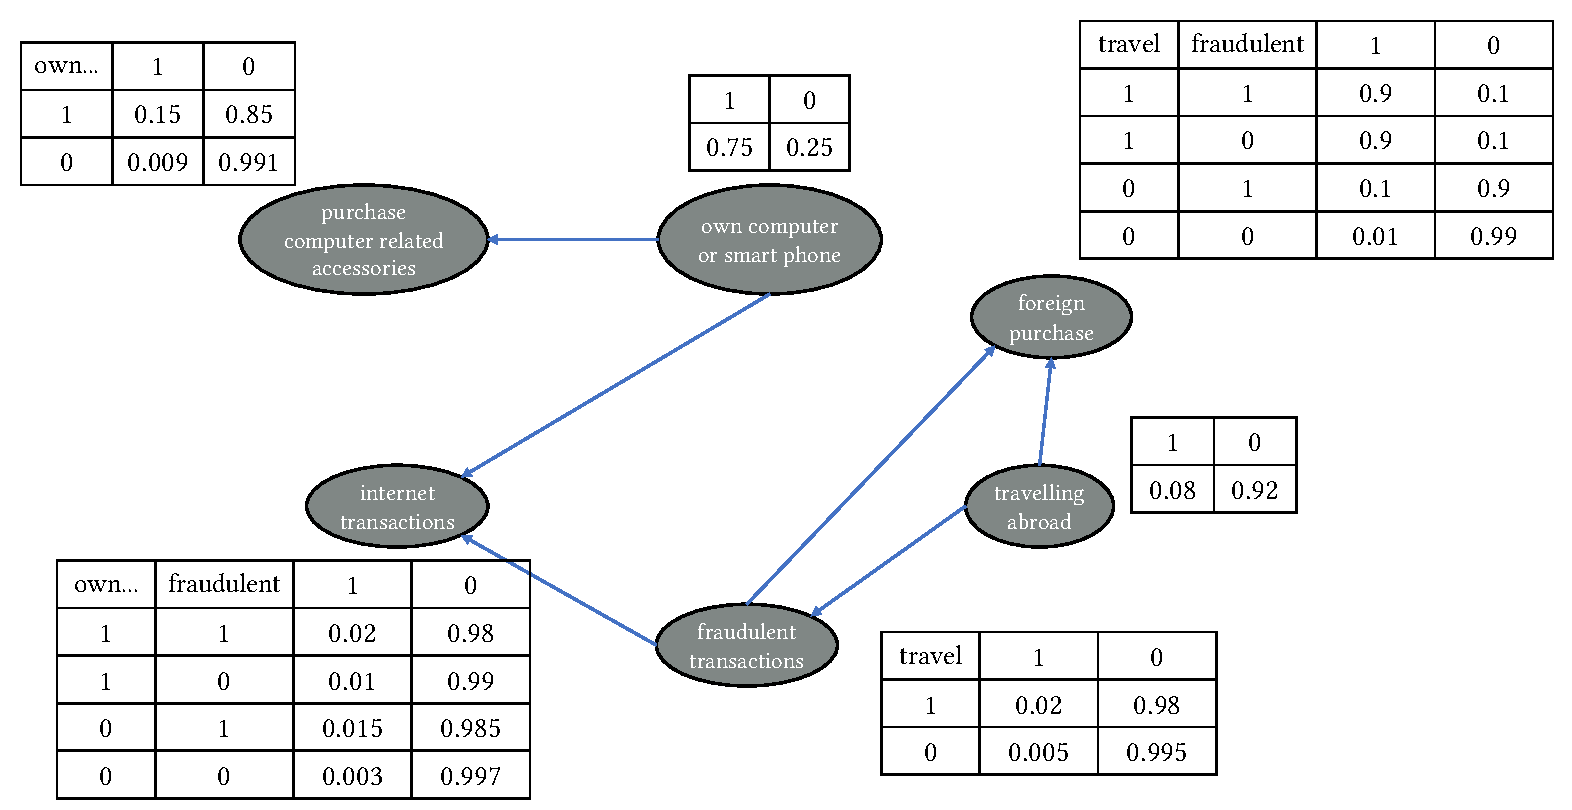
\includegraphics[width=0.8\textwidth]{figures/q4.pdf}
	\caption{Bayes Network to Question \#4}
	\label{fig:q4}
\end{figure}

\subsection{Answer to Question \#4.2}


The prior probability that the current transaction is legitimate is 0.9938. The calculation is as follows:

Abbreviations: $fraudulent \to fr, travel \to tr$
\begin{equation}
	\begin{aligned}
		& P(fr=0)=\sum_{tr} P(fr=0|tr) = 0.08 \times 0.98 +0.92 \times 0.995=0.9938\\
	\end{aligned}
\end{equation}


The probability that the current transaction is a legitimate one is 0.98726326. The calculation is as follows:

Abbreviations: $fraudulent \to fr, travel \to tr, foreign\_purchase \to fp,internet\_purchase \to ip, \\ purchase\_computer \to pc, own\_computer \to oc$
\begin{equation}
	\begin{aligned}
		& P(fr=0|fp=0, ip=1, pc=1) = \frac{P(fr=0, fp=0, ip=1, pc=1)}{P(fp=0, ip=1, pc=1)} \\
		& = \frac{\sum_{oc} \sum_{tr} P(oc)P(tr)P(fr=0|tr)P(fp=0|fr=0,tr)P(ip=1|fr=0,oc)P(pc=1|oc)}{\sum_{oc} \sum_{tr} \sum_{fr} P(oc)P(tr)P(fr|tr)P(fp=0|fr,tr)P(ip=1|fr,oc)P(pc=1|oc)} \\
		& = \frac{\sum_{oc} P(oc)P(ip=1|fr=0,oc)P(pc=1|oc) \sum_{tr} P(tr)P(fr=0|tr)P(fp=0|fr=0,tr)}{\splitfrac{\sum_{oc} \sum_{tr} P(oc)P(tr)P(fr=0|tr)P(fp=0|fr=0,tr)P(ip=1|fr=0,oc)P(pc=1|oc)}{+ \sum_{oc} \sum_{tr} P(oc)P(tr)P(fr=1|tr)P(fp=0|fr=1,tr)P(ip=1|fr=1,oc)P(pc=1|oc)}} \\
		& = \frac{(0.01\times0.75+0.003\times0.25)\times(0.15\times0.75+0.009\times0.25)\times(0.08 \times 0.98 +0.92 \times 0.995)\times(0.1 \times 0.08+0.99\times0.92)}{\splitfrac{(0.08 \times 0.98 +0.92 \times 0.995)\times(0.1 \times 0.08+0.99\times0.92)\times(0.01\times0.75+0.003\times0.25)\times(0.15\times0.75+0.009\times0.25)}{+(0.02 \times0.08+0.92\times0.005)\times(0.1\times0.08+0.9\times0.92)\times(0.02\times0.75+0.015\times0.25)\times(0.15\times0.75+0.009\times0.25)} } \\
		& = \frac{0.0008644236129}{0.0008755755916} = 0.98726326 \\
	\end{aligned}
\end{equation}

\subsection{Answer to Question \#4.3}
As her spouse confirms that she is currently traveling, i.e, $tr=1$, the probability that the current transaction is legitimate would reduce into 0.9556737589, i.e., the probability of a fraud increases a bit. The calculation is as follows:
\begin{equation}
	\begin{aligned}
		& P(fr=0|fp=0, ip=1, pc=1, tr=1) = \frac{P(fr=0, fp=0, ip=1, pc=1, tr=1)}{P(fp=0, ip=1, pc=1, tr=1)} \\
		& = \frac{\sum_{oc} P(oc)P(fr=0|tr=1)P(fp=0|fr=0,tr=1)P(ip=1|fr=0,oc)P(pc=1|oc)}{\sum_{oc} \sum_{fr} P(oc)P(fr|tr=1)P(fp=0|fr,tr=1)P(ip=1|fr,oc)P(pc=1|oc)} \\
		& = \frac{0.98\times0.1\times(0.01\times0.75+0.003\times0.25)\times(0.15\times0.75+0.009\times0.25)}{\splitfrac{0.98\times0.1\times(0.01\times0.75+0.003\times0.25)\times(0.15\times0.75+0.009\times0.25)}{+0.02\times0.1\times(0.02\times0.75+0.015\times0.25)\times(0.15\times0.75+0.009\times0.25)}} \\
		& =\frac{0.000092775375}{0.0000970785} = 0.9556737589 \\
	\end{aligned}
\end{equation}

\section{Question \#5}
The Most Probable Explanation for $G=g1$ and $L=l0$ is $I=i1$, $D=d0$, and $S=s1$. The probability is 0.01296. The calculation is as follows:

The joint distribution of the given Bayesian network is $P(I,D,G,S,L) = P(I) P(D) P(G|I,D) P(S|I) P(L|G)$.
\begin{itemize}[leftmargin=*]
	\setlength{\itemsep}{0pt}
	\setlength{\parsep}{0pt}
	\setlength{\parskip}{0pt}
	\item \textbf{Forward pass:}
\begin{equation}
	\begin{aligned}
		& \max_{D,I,S} P(I,D,G=g1,S,L=l0)\\
		&= \max_{D,I,S} P(I)P(D)P(G=g1|I, D)P(S|I)P(L=l0|G=g1)\\
		&= \max_{I} P(I) \max_D P(D)P(G=g1|I, D) \max_S P(S|I) * 0.1 \\
		&= \max_{I} \left[ \begin{array}{cc}
			i0 & i1\\
			0.7 & 0.3
			\end{array}\right] 
			\left[ \begin{array}{cc}
			i0 & i1\\
			0.18 & 0.54
			\end{array}\right] 
			\left[ \begin{array}{cc}
			i0 & i1\\
			0.95 & 0.8
			\end{array}\right]* 0.1 \\
		&= \max_{I} \left[ \begin{array}{cc}
			i0 & i1\\
			0.01197 & 0.01296
			\end{array}\right] = 0.01296 \\
	\end{aligned}
\end{equation}
	\item \textbf{Backward pass:} $MPE = \arg\max_{D,I,S} P(I,D,G=g1,S,L=l0) = (I=i1, D=d0, S=s1)$, i.e., the most probable explanation for $G=g1$ and $L=l0$ is $I=i1$, $D=d0$, and $S=s1$.
\end{itemize}

\section{Question \#6}

\begin{table}[!h]
	\centering
	\caption{MDP model in Question \#6}
	\label{tab:q6}
	\begin{tabular}{@{}ccccc@{}}
	\toprule
	State & Action   & State$^{\prime}$ & $P(s^{\prime}|s, a)$ & $Reward(s,a,s^{\prime})$ \\ \midrule
	L1    & Pickup   & L1     & 0.7       & 0              \\
	L1    & Pickup   & L2     & 0.15      & 19             \\
	L1    & Pickup   & L3     & 0.09     & 8.5           \\
	L1    & Pickup   & L4     & 0.06       & 7.75          \\
	L1    & MoveToL2 & L2     & 1         & -1             \\
	L1    & MoveToL3 & L3     & 1         & -1.5           \\
	L1    & MoveToL4 & L4     & 1         & -1.25          \\
	L2    & Pickup   & L2     & 0.5       & 0              \\
	L2    & Pickup   & L1     & 0.2      & 9          \\
	L2    & Pickup   & L3     & 0.3      & 6.25           \\
	L2    & MoveToL1 & L1     & 1         & -1             \\
	L2    & MoveToL3 & L3     & 1         & -1.75          \\
	L3    & Pickup   & L3     & 0.4       & 0              \\
	L3    & Pickup   & L1     & 0.18       & 13.5           \\
	L3    & Pickup   & L4     & 0.42       & 7.8            \\
	L3    & MoveToL1 & L1     & 1         & -1.5           \\
	L3    & MoveToL4 & L4     & 1         & -1.2           \\
	L4    & Pickup   & L4     & 0.2       & 0              \\
	L4    & Pickup   & L1     & 0.32       & 9.75           \\
	L4    & Pickup   & L2     & 0.48       & 4              \\
	L4    & MoveToL1 & L1     & 1         & -1.25          \\
	L4    & MoveToL2 & L2     & 1         & -1             \\ \bottomrule
	\end{tabular}
	\end{table}

\subsection{Answer to Question \#6.a}
The MDP model is defined as follows:
\begin{itemize}[leftmargin=*]
	\setlength{\itemsep}{0pt}
	\setlength{\parsep}{0pt}
	\setlength{\parskip}{0pt}
	\item \textbf{States}: $S = \{L1, L2, L3, L4\}$.
	\item \textbf{Actions}: $A = \{Pickup, MoveToL1, MoveToL2, MoveToL3, MoveToL4\}$
	\item \textbf{transition probability matrices}: Shown in the fourth column of Table~\ref{tab:q6}.
	\item \textbf{Reward function}: Shown in the fifth column of Table~\ref{tab:q6}.
\end{itemize}


\subsection{Answer to Question \#6.b}

The code is shown below, as well as available from this link.

Figure \ref{fig:q6b} shows the two steps of value iteration in the solution.

\end{document}
